\documentclass{../../csbeamer}

% Add theme and color scheme
% \usetheme{Madrid}
% \usecolortheme{dolphin}
% \useinnertheme{circles}

% % Add transition options for the whole presentation
% \setbeamercovered{transparent}
% \setbeamertemplate{navigation symbols}{}

% % Add custom animation commands
% \usepackage{tikz}
% \usepackage{animate}
% \usepackage{verbatim}

% Add custom color definitions for consistency
\definecolor{robotblue}{HTML}{4285F4}
\definecolor{robotred}{HTML}{EA4335}
\definecolor{robotgreen}{HTML}{34A853}
\definecolor{robotyellow}{HTML}{FBBC05}

\university{St. Francis Xavier University}
\department{Department of Computer Science}
\course{CSCI-529 - Mobile Robotics}
\courseshort{CSCI-529 - Robotics}
\term{Fall 2025}
\author{Dr. Jean-Alexis Delamer}

\title{Robot Kinematics}

\begin{document}

\frame{\titlepage}

% Section: Kinematics
\section{Kinematics}

% Subsection: Introduction to Kinematics
\subsection{Introduction to Kinematics}

\begin{frame}
    \frametitle{Introduction to Kinematics}
    \begin{block}<1->{What is Kinematics?}
        \textbf{Kinematics} is the study of how things move, focusing on position, velocity, and acceleration, without considering the forces that cause the motion.
    \end{block}
    
    \onslide<2->{
    In robotics, kinematics helps us answer: 
    \begin{center}
        \textcolor{robotblue}{"Given certain wheel speeds, where will the robot go?"}
    \end{center}
    }
    
    \begin{block}<3->{Why is it important?}
        \begin{itemize}
            \item<3-> \textcolor{robotgreen}{Essential} for programming robot movement
            \item<4-> \textcolor{robotblue}{Foundation} for navigation and control
            \item<5-> \textcolor{robotred}{Used} in simulation and real-world robots
        \end{itemize}
    \end{block}
    
\end{frame}

% Subsection: Kinematics vs. Dynamics
\subsection{Kinematics vs. Dynamics}
\begin{frame}
    \frametitle{Kinematics vs. Dynamics}
    \begin{columns}
        \begin{column}{0.5\textwidth}
            \begin{block}<1->{Kinematics}
                \begin{itemize}
                    \item<1-> Studies \textcolor{robotblue}{motion only}
                    \item<2-> Position, velocity, acceleration
                    \item<3-> "What path does the robot follow?"
                \end{itemize}
            \end{block}
            
            \begin{block}<4->{Dynamics}
                \begin{itemize}
                    \item<4-> Studies \textcolor{robotred}{forces and torques}
                    \item<5-> Mass, inertia, friction
                    \item<6-> "Why does the robot move this way?"
                \end{itemize}
            \end{block}
        \end{column}
        
        \begin{column}{0.5\textwidth}
            \only<1-3>{
                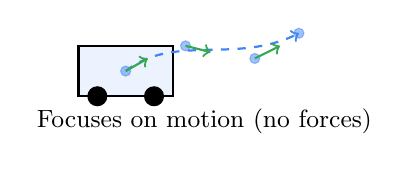
\begin{tikzpicture}[scale=0.8]
                    % Kinematics illustration
                    \draw[thick, fill=robotblue!10] (0,0) rectangle (1.5,0.8);
                    \draw[fill=black] (0.3,0) circle (0.15);
                    \draw[fill=black] (1.2,0) circle (0.15);
                    
                    % Path
                    \draw[->, thick, dashed, robotblue] (0.75,0.4) .. controls (1.5,1) and (2.5,0.5) .. (3.5,1);
                    
                    % Position markers
                    \filldraw[robotblue, opacity=0.5] (0.75,0.4) circle (0.08);
                    \filldraw[robotblue, opacity=0.5] (1.7,0.8) circle (0.08);
                    \filldraw[robotblue, opacity=0.5] (2.8,0.6) circle (0.08);
                    \filldraw[robotblue, opacity=0.5] (3.5,1) circle (0.08);
                    
                    % Velocity vectors (shown with small arrows)
                    \draw[->, thick, robotgreen] (0.75,0.4) -- (1.1,0.6);
                    \draw[->, thick, robotgreen] (1.7,0.8) -- (2.1,0.7);
                    \draw[->, thick, robotgreen] (2.8,0.6) -- (3.2,0.8);
                    
                    \node at (2,-0.4) {\small{Focuses on motion (no forces)}};
                \end{tikzpicture}
            }
            
            \only<4-6>{
                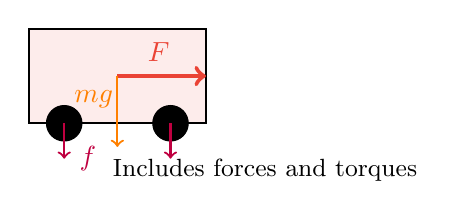
\begin{tikzpicture}[scale=1.5]
                    % Dynamics illustration
                    \draw[thick, fill=robotred!10] (0,0) rectangle (1.5,0.8);
                    \draw[fill=black] (0.3,0) circle (0.15);
                    \draw[fill=black] (1.2,0) circle (0.15);
                    
                    % Force vectors
                    \draw[->, ultra thick, robotred] (0.75,0.4) -- (1.5,0.4);
                    \node[robotred] at (1.1,0.6) {$F$};
                    
                    % Weight force
                    \draw[->, thick, orange] (0.75,0.4) -- (0.75,-0.2);
                    \node[orange] at (0.55,0.2) {$mg$};
                    
                    % Friction force
                    \draw[->, thick, purple] (0.3,0) -- (0.3,-0.3);
                    \draw[->, thick, purple] (1.2,0) -- (1.2,-0.3);
                    \node[purple] at (0.5,-0.3) {$f$};
                    
                    \node at (2,-0.4) {\small{Includes forces and torques}};
                \end{tikzpicture}
            }
        \end{column}
    \end{columns}
    
    \only<7->{
        \begin{center}
            \textit{In this course, we focus primarily on kinematics for mobile robots.}
        \end{center}
    }
\end{frame}

% Subsection: Kinematic Models Overview
\subsection{Kinematic Models Overview}
\begin{frame}
    \frametitle{Kinematic Models Overview}
    \begin{columns}
        \begin{column}{0.55\textwidth}
            \begin{block}<1->{Common Robot Drive Systems}
                \begin{itemize}
                    \item<1-> \textcolor{robotblue}{Differential Drive:} Two independently driven wheels
                    \item<2-> \textcolor{robotgreen}{Omnidirectional Drive:} Movement in any direction
                    \item<3-> \textcolor{robotyellow}{Ackermann Steering:} Car-like steering
                \end{itemize}
            \end{block}
            
            \begin{block}<4->{Example Robots}
                \begin{itemize}
                    \item<4-> Differential: TurtleBot, Roomba
                    \item<5-> Omnidirectional: Mecanum-wheeled robots
                    \item<6-> Ackermann: Self-driving cars, RC cars
                \end{itemize}
            \end{block}
        \end{column}
        
        \begin{column}{0.45\textwidth}
            \only<1>{
                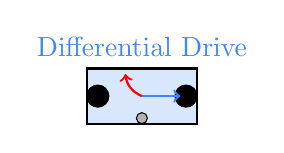
\begin{tikzpicture}[scale=0.7]
                    % Differential drive - corrected to have exactly two wheels
                    \draw[thick, fill=robotblue!20] (0,0) rectangle (2,1);
                    % Left wheel
                    \draw[fill=black] (0.2,0.5) circle (0.2);
                    % Right wheel
                    \draw[fill=black] (1.8,0.5) circle (0.2);
                    % Caster wheel (smaller)
                    \draw[fill=gray!60] (1,0.1) circle (0.1);
                    % Direction arrows
                    \draw[->, thick, robotblue] (1,0.5) -- (1.7,0.5);
                    \draw[->, thick, red] (1,0.5) to[bend left] (0.7,0.9);
                    \node[robotblue] at (1,1.4) {Differential Drive};
                \end{tikzpicture}
            }
            \only<2>{
                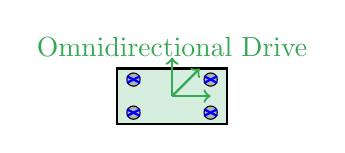
\begin{tikzpicture}[scale=0.7]
                    % Omnidirectional
                    \draw[thick, fill=robotgreen!20] (0,0) rectangle (2,1);
                    % Mecanum wheels
                    \foreach \x/\y in {0.3/0.2, 0.3/0.8, 1.7/0.2, 1.7/0.8} {
                        \draw[fill=gray!60] (\x,\y) circle (0.12);
                        \draw[thick, blue] (\x-0.12,\y-0.06) -- (\x+0.12,\y+0.06);
                        \draw[thick, blue] (\x-0.12,\y+0.06) -- (\x+0.12,\y-0.06);
                    }
                    % Movement arrows
                    \draw[->, thick, robotgreen] (1,0.5) -- (1.7,0.5);
                    \draw[->, thick, robotgreen] (1,0.5) -- (1,1.2);
                    \draw[->, thick, robotgreen] (1,0.5) -- (1.5,1.0);
                    \node[robotgreen] at (1,1.4) {Omnidirectional Drive};
                \end{tikzpicture}
            }
            \only<3>{
                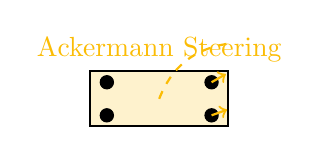
\begin{tikzpicture}[scale=0.7]
                    % Ackermann steering
                    \draw[thick, fill=robotyellow!20] (0,0) rectangle (2.5,1);
                    % Wheels
                    \draw[fill=black] (0.3,0.2) circle (0.12);
                    \draw[fill=black] (0.3,0.8) circle (0.12);
                    \draw[fill=black] (2.2,0.2) circle (0.12);
                    \draw[fill=black] (2.2,0.8) circle (0.12);
                    % Steering
                    \draw[->, thick, robotyellow, rotate around={20:(2.2,0.2)}] (2.2,0.2) -- (2.5,0.2);
                    \draw[->, thick, robotyellow, rotate around={30:(2.2,0.8)}] (2.2,0.8) -- (2.5,0.8);
                    % Motion path
                    \draw[thick, dashed, robotyellow] (1.25,0.5) to[bend left=30] (2.5,1.5);
                    \node[robotyellow] at (1.25,1.4) {Ackermann Steering};
                \end{tikzpicture}
            }
            \only<4-6>{
                \begin{tikzpicture}[scale=0.65]
                    % Example robot images as stylized drawings
                    \only<4>{
                        % TurtleBot-like robot
                        \draw[thick, fill=robotblue!20] (0,0) circle (1.5);
                        \draw[thick, fill=robotblue!30] (0,0) circle (1);
                        \draw[thick, fill=white] (0,0) circle (0.7);
                        \draw[fill=black] (-0.8,-1.3) circle (0.2);
                        \draw[fill=black] (0.8,-1.3) circle (0.2);
                        \draw[thick, ->] (0,0) -- (0,1.2);
                        \node at (0,1.9) {TurtleBot};
                    }
                    \only<5>{
                        % Mecanum robot
                        \draw[thick, fill=robotgreen!20] (-1.5,-1) rectangle (1.5,1);
                        \foreach \x/\y in {-1.2/-0.8, -1.2/0.8, 1.2/-0.8, 1.2/0.8} {
                            \draw[fill=gray!60] (\x,\y) circle (0.25);
                            \draw[thick, blue, rotate around={45:(\x,\y)}] (\x-0.25,\y) -- (\x+0.25,\y);
                            \draw[thick, blue, rotate around={135:(\x,\y)}] (\x-0.25,\y) -- (\x+0.25,\y);
                        }
                        \node at (0,1.5) {Mecanum Robot};
                    }
                    \only<6>{
                        % Car-like robot with improved proportions
                        \draw[thick, fill=robotyellow!20] (-1.7,-0.8) rectangle (1.7,0.5);
                        % Car front (hood/cabin)
                        \draw[thick, fill=robotyellow!30] (-0.2,0.5) rectangle (1.7,1.1);
                        % Wheels with better positioning
                        \draw[fill=black] (-1.3,-0.8) circle (0.3);
                        \draw[fill=black] (1.3,-0.8) circle (0.3);                       
                        \draw[thick] (0.7,0.8) circle (0.2);
                        \draw[thick] (0.7,0.8) -- (0.7,0.6);
                        \draw[thick] (0.7,0.8) -- (0.5,0.8);
                        \node at (0,1.8) {Car-like Robot};
                    }
                \end{tikzpicture}
            }
        \end{column}
    \end{columns}
\end{frame}

\begin{frame}
    \frametitle{Figure: Kinematic Models}
    \begin{center}
    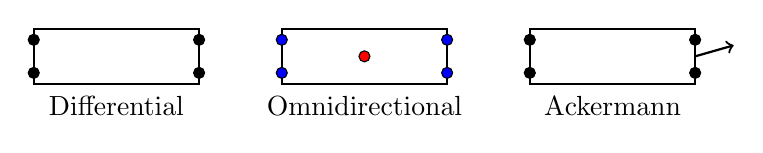
\begin{tikzpicture}[scale=0.7]
    % Differential drive
    \draw[thick] (0,0) rectangle (3,1);
    \draw[fill=black] (0,0.2) circle (0.1);
    \draw[fill=black] (0,0.8) circle (0.1);
    \draw[fill=black] (3,0.2) circle (0.1);
    \draw[fill=black] (3,0.8) circle (0.1);
    \node at (1.5,-0.4) {Differential};
    % Omnidirectional
    \begin{scope}[shift={(4.5,0)}]
        \draw[thick] (0,0) rectangle (3,1);
        \foreach \x in {0,3} {\foreach \y in {0.2,0.8} {\draw[fill=blue] (\x,\y) circle (0.1);}}
        \draw[fill=red] (1.5,0.5) circle (0.1);
        \node at (1.5,-0.4) {Omnidirectional};
    \end{scope}
    % Ackermann
    \begin{scope}[shift={(9,0)}]
        \draw[thick] (0,0) rectangle (3,1);
        \draw[fill=black] (0,0.2) circle (0.1);
        \draw[fill=black] (0,0.8) circle (0.1);
        \draw[fill=black] (3,0.2) circle (0.1);
        \draw[fill=black] (3,0.8) circle (0.1);
        \draw[thick,->] (3,0.5) -- (3.7,0.7);
        \node at (1.5,-0.4) {Ackermann};
    \end{scope}
    \end{tikzpicture}
    \end{center}
    \small{(Schematic representations of three common mobile robot kinematic models)}
\end{frame}

% Subsection: Coordinate Systems
\subsection{Coordinate Systems in Robotics}
\begin{frame}
    \frametitle{Coordinate Systems in Robotics}
    \begin{columns}
        \begin{column}{0.55\textwidth}
            \begin{block}<1->{World (Global) Frame}
                \begin{itemize}
                    \item<1-> Fixed reference frame (e.g., map or room)
                    \item<2-> Used for absolute positioning
                    \item<3-> Does not move with the robot
                \end{itemize}
            \end{block}
            
            \begin{block}<4->{Robot (Body) Frame}
                \begin{itemize}
                    \item<4-> Attached to the robot's center
                    \item<5-> Moves and rotates with the robot
                    \item<6-> Used for local sensing and control
                \end{itemize}
            \end{block}
        \end{column}
        
        \begin{column}{0.45\textwidth}
            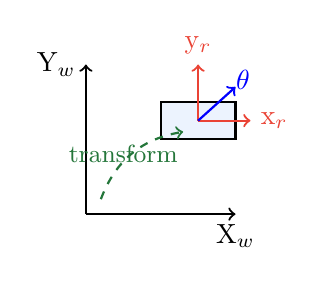
\begin{tikzpicture}[scale=0.95]
                % World frame axes
                \draw<1->[->, thick] (0,0) -- (2,0) node[below] {X$_w$};
                \draw<1->[->, thick] (0,0) -- (0,2) node[left] {Y$_w$};
                
                % Robot body - appears on slide 4
                \draw<4->[thick, fill=robotblue!10] (1,1) rectangle (2,1.5);
                
                % Robot frame axes - appears on slide 4
                \draw<4->[->, thick, robotred] (1.5,1.25) -- (2.2,1.25) node[right, robotred] {x$_r$};
                \draw<4->[->, thick, robotred] (1.5,1.25) -- (1.5,2) node[above, robotred] {y$_r$};
                
                % Heading angle - appears on slide 6
                \draw<6->[->, thick, blue] (1.5,1.25) -- (2,1.7);
                \node<6->[blue] at (2.1,1.8) {$\theta$};
                
                % Transformation arrows - appears on slide 7
                \draw<7->[thick, ->, dashed, robotgreen!70!black] (0.2,0.2) to[bend left] (1.3,1.1);
                \node<7->[robotgreen!70!black, font=\small] at (0.5,0.8) {transform};
            \end{tikzpicture}
            
            \only<8->{
                \vspace{0.5cm}
                \begin{align*}
                    \begin{bmatrix} x_w \\ y_w \\ 1 \end{bmatrix} &= 
                    \begin{bmatrix} 
                    \cos\theta & -\sin\theta & x_r \\ 
                    \sin\theta & \cos\theta & y_r \\ 
                    0 & 0 & 1
                    \end{bmatrix}
                    \begin{bmatrix} x_r \\ y_r \\ 1 \end{bmatrix}
                \end{align*}
            }
        \end{column}
    \end{columns}
\end{frame}

% Subsection: Degrees of Freedom
\subsection{Degrees of Freedom (DoF)}
\begin{frame}
    \frametitle{Degrees of Freedom (DoF)}
    \textbf{Definition:} The number of independent parameters that define the robot's configuration.
    \begin{itemize}
        \item In 2D: typically $x$, $y$, and $\theta$ (3 DoF)
        \item A car-like robot: 3 DoF, but only 2 can be controlled directly (nonholonomic)
        \item A holonomic robot (e.g., omnidirectional): can control all 3 DoF
    \end{itemize}
    \textbf{Why it matters:}
    \begin{itemize}
        \item Determines what motions are possible
        \item Affects path planning and control
    \end{itemize}
\end{frame}

% Subsection: Kinematic Constraints
\subsection{Kinematic Constraints}
\begin{frame}
    \frametitle{Kinematic Constraints}
    \textbf{Holonomic:} All degrees of freedom can be controlled independently.
    
    \textbf{Nonholonomic:} Some constraints limit motion (e.g., a car cannot move sideways).
    \begin{itemize}
        \item Most mobile robots are nonholonomic.
        \item Impacts path planning and control.
    \end{itemize}
\end{frame}

% Subsection: Differential Drive Kinematics
\subsection{Differential Drive Kinematics}
\begin{frame}
    \frametitle{Differential Drive Kinematics}
    \begin{columns}
        \begin{column}{0.5\textwidth}
            \begin{block}<1->{The Model}
                \begin{itemize}
                    \item<1-> Two individually controlled wheels
                    \item<2-> Wheels share a common axis
                    \item<3-> Often includes a third support wheel
                \end{itemize}
            \end{block}
            
            \begin{block}<4->{Parameters}
                \begin{itemize}
                    \item<4-> $r_L$: Left wheel velocity
                    \item<5-> $r_R$: Right wheel velocity
                    \item<6-> $d$: Distance between wheels
                \end{itemize}
            \end{block}
        \end{column}
        
        \begin{column}{0.5\textwidth}
            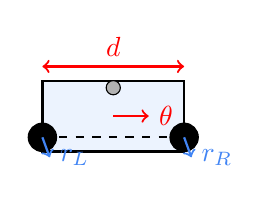
\begin{tikzpicture}[scale=0.9]
                % Draw the robot chassis
                \draw<1->[thick, fill=robotblue!10] (0,0) rectangle (2,1);
                
                % Draw wheels
                \draw<2->[fill=black] (0,0.2) circle (0.2);
                \draw<2->[fill=black] (2,0.2) circle (0.2);
                
                % Draw axle
                \draw<2->[thick, dashed] (0,0.2) -- (2,0.2);
                
                % Draw caster wheel
                \draw<3->[fill=gray!60] (1,0.9) circle (0.1);
                
                % Add labels when parameters are introduced
                \draw<4->[<->, thick, red] (0,1.2) -- (2,1.2) node[midway, above] {$d$};
                
                % Show rotation arrows for wheels when velocities introduced
                \draw<5->[->, thick, robotblue, rotate around={-70:(0,0.2)}] (0,0.2) -- (0.3,0.2) node[right] {$r_L$};
                \draw<6->[->, thick, robotblue, rotate around={-70:(2,0.2)}] (2,0.2) -- (2.3,0.2) node[right] {$r_R$};
                
                % Add robot heading at the end
                \draw<7->[->, thick, red] (1,0.5) -- (1.5,0.5) node[right] {$\theta$};
            \end{tikzpicture}
            
            \only<7->{
                \begin{align*}
                    v &= \frac{r_L + r_R}{2} \\
                    \omega &= \frac{r_R - r_L}{d}
                \end{align*}
            }
        \end{column}
    \end{columns}
\end{frame}

% Subsection: Kinematic Equations
\subsection{Kinematic Equations}
\begin{frame}
    \frametitle{Kinematic Equations and Applications}
    \textbf{How do we predict where the robot will be after some time?}
    
    Use the robot's linear and angular velocity to update its position and orientation.
\end{frame}

\begin{frame}
    \frametitle{Where Do the General Kinematic Equations Come From?}
    The general kinematic equations for a mobile robot describe how its position $(x, y)$ and orientation $\theta$ change over time, given its linear velocity $v$ and angular velocity $\omega$.
    
    \textbf{Assumptions:}
    \begin{itemize}
        \item The robot moves in a 2D plane.
        \item $v$ is the forward speed (along the robot's heading).
        \item $\omega$ is the rate of rotation (change in heading).
    \end{itemize}
    
    \textbf{Key idea:} At any instant, the robot moves forward by $v \cdot dt$ in the direction of its current heading $\theta$.
\end{frame}

\begin{frame}
    \frametitle{Derivation of the Kinematic Equations}
    \begin{columns}
        \begin{column}{0.6\textwidth}
            \begin{block}{Robot's Motion Equations}
                \begin{align*}
                    \frac{dx}{dt} &= v \cos(\theta) \\
                    \frac{dy}{dt} &= v \sin(\theta) \\
                    \frac{d\theta}{dt} &= \omega
                \end{align*}
            \end{block}
            \begin{block}<3->{Explanation}
                \begin{itemize}
                    \item<3-> $\frac{dx}{dt}$ and $\frac{dy}{dt}$ are rates of change in position
                    \item<5-> $\frac{d\theta}{dt}$ is rate of orientation change
                \end{itemize}
            \end{block}
        \end{column}
        
        \begin{column}{0.4\textwidth}
            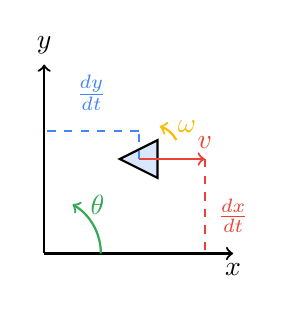
\begin{tikzpicture}[scale=1.2]
                % Axes
                \draw<1->[->, thick] (0,0) -- (2,0) node[below] {$x$};
                \draw<1->[->, thick] (0,0) -- (0,2) node[above] {$y$};
                
                % Robot (triangle)
                \draw<2->[thick, fill=robotblue!20] (0.8,1) -- (1.2,1.2) -- (1.2,0.8) -- cycle;
                
                % Velocity vector
                \draw<2->[->, thick, robotred] (1,1) -- (1.7,1) node[above] {$v$};
                
                % Angle theta
                \draw<2->[thick, robotgreen, ->] (0.6,0) arc (0:60:0.6) node[right=1mm] {$\theta$};
                
                % Angular velocity
                \draw<5->[thick, ->, robotyellow, rotate around={28:(1.4,1.2)}] (1.4,1.2) arc (0:45:0.3) node[right=1mm] {$\omega$};
                
                % dx/dt and dy/dt components
                \draw<3->[dashed, thick, robotred] (1,01) -- (1.7,1);
                \draw<3->[dashed, thick, robotred] (1.7,1) -- (1.7,0);
                \node<3->[robotred] at (2,0.4) {$\frac{dx}{dt}$};
                
                \draw<4->[dashed, thick, robotblue] (1,1) -- (1,1.3);
                \draw<4->[dashed, thick, robotblue] (1,1.3) -- (0,1.3);
                \node<4->[robotblue] at (0.5,1.7) {$\frac{dy}{dt}$};
            \end{tikzpicture}
            
            \only<6->{
                \begin{align*}
                    \begin{pmatrix} x(t) \\ y(t) \\ \theta(t) \end{pmatrix} &= 
                    \begin{pmatrix} 
                    x(0) + v \cos(\theta) t \\
                    y(0) + v \sin(\theta) t \\
                    \theta(0) + \omega t
                    \end{pmatrix}
                \end{align*}
            }
        \end{column}
    \end{columns}
\end{frame}

\begin{frame}
    \frametitle{General Kinematic Equations}
    \begin{align*}
        x(t) &= x(0) + v \cdot \cos(\theta) \cdot t \\
        y(t) &= y(0) + v \cdot \sin(\theta) \cdot t \\
        \theta(t) &= \theta(0) + \omega \cdot t
    \end{align*}
    \textbf{Where:}
    \begin{itemize}
        \item $(x, y)$: robot position
        \item $\theta$: orientation (heading)
        \item $v$: linear velocity
        \item $\omega$: angular velocity
    \end{itemize}
\end{frame}

\begin{frame}
    \frametitle{Non-Constant Velocities}
    In real robots, $v$ and $\omega$ often change over time.
    \begin{itemize}
        \item If $v(t)$ and $\omega(t)$ are piecewise constant, update pose in small time steps.
        \item For general $v(t)$ and $\omega(t)$, integrate numerically:
    \end{itemize}
    \begin{align*}
        x(t+\Delta t) &= x(t) + v(t) \cos(\theta(t)) \Delta t \\
        y(t+\Delta t) &= y(t) + v(t) \sin(\theta(t)) \Delta t \\
        \theta(t+\Delta t) &= \theta(t) + \omega(t) \Delta t
    \end{align*}
    \small{(Used in simulation and real robot control)}
\end{frame}

% Subsection: Path Following and Trajectory Tracking
\subsection{Path Following and Trajectory Tracking}
\begin{frame}
    \frametitle{Path Following and Trajectory Tracking}
    \begin{columns}
        \begin{column}{0.55\textwidth}
            \begin{block}<1->{Path Following}
                \begin{itemize}
                    \item<1-> Move along a \textcolor{robotblue}{geometric path}
                    \item<2-> Focus on spatial accuracy
                    \item<3-> No timing constraints
                \end{itemize}
            \end{block}
            
            \begin{block}<4->{Trajectory Tracking}
                \begin{itemize}
                    \item<4-> Follow a path with \textcolor{robotred}{specific timing}
                    \item<5-> Must be at certain locations at certain times
                    \item<6-> More challenging but necessary for coordination
                \end{itemize}
            \end{block}
        \end{column}
        
        \begin{column}{0.45\textwidth}
            \begin{tikzpicture}[scale=0.9]
                % Path for both demonstrations
                \draw<1->[thick, robotblue] (0,0) .. controls (1,1) and (2,0.5) .. (3,1.5);
                
                % Path following demonstration
                \only<1-3>{
                    % Robot at different points with no timing markers
                    \draw<1->[thick, fill=robotblue!10] (0,0) rectangle (0.4,0.2);
                    \draw<1->[->, thick, red] (0.2,0.1) -- (0.5,0.2);
                    
                    \draw<2->[thick, fill=robotblue!10] (1.5,0.7) rectangle (1.9,0.9);
                    \draw<2->[->, thick, red] (1.7,0.8) -- (2.0,0.9);
                    
                    \draw<3->[thick, fill=robotblue!10] (3,1.5) rectangle (3.4,1.7);
                    \draw<3->[->, thick, red] (3.2,1.6) -- (3.5,1.7);
                }
                
                % Trajectory tracking demonstration
                \only<4-6>{
                    % Robot at different points with timing markers
                    \draw<4->[thick, fill=robotred!10] (0,0) rectangle (0.4,0.2);
                    \draw<4->[->, thick, red] (0.2,0.1) -- (0.5,0.2);
                    \node<4->[robotred] at (0.2,-0.3) {t = 0s};
                    
                    \draw<5->[thick, fill=robotred!10] (1.5,0.7) rectangle (1.9,0.9);
                    \draw<5->[->, thick, red] (1.7,0.8) -- (2.0,0.9);
                    \node<5->[robotred] at (1.7,0.3) {t = 5s};
                    
                    \draw<6->[thick, fill=robotred!10] (3,1.5) rectangle (3.4,1.7);
                    \draw<6->[->, thick, red] (3.2,1.6) -- (3.5,1.7);
                    \node<6->[robotred] at (3.2,1.2) {t = 10s};
                }
            \end{tikzpicture}
        \end{column}
    \end{columns}
\end{frame}

% Subsection: Inverse Kinematics
\subsection{Inverse Kinematics}
\begin{frame}
    \frametitle{Inverse Kinematics: From Trajectory to Wheel Velocities}
    \textbf{Problem:} Given a desired $v$ and $\omega$, what should the wheel velocities be?
    \begin{align*}
        r_L &= v - \frac{d}{2} \omega \\
        r_R &= v + \frac{d}{2} \omega
    \end{align*}
    \begin{itemize}
        \item $d$ is the distance between wheels
        \item Used to convert planned motion into motor commands
    \end{itemize}
    \textbf{Example:} If $v=0.3$ m/s, $\omega=0.2$ rad/s, $d=0.5$ m:
    \begin{itemize}
        \item $r_L = 0.3 - 0.25 \times 0.2 = 0.25$ m/s
        \item $r_R = 0.3 + 0.25 \times 0.2 = 0.35$ m/s
    \end{itemize}
\end{frame}

% Subsection: Simulating Robot Motion
\subsection{Simulating Robot Motion}
\begin{frame}[fragile]
    \frametitle{Simulating Robot Motion (Pseudocode)}
    \textbf{Numerical integration for robot pose:}
    \begin{verbatim}
    x, y, theta = x0, y0, theta0
    for t in range(0, T, dt):
        x += v * cos(theta) * dt
        y += v * sin(theta) * dt
        theta += omega * dt
    \end{verbatim}
    \begin{itemize}
        \item Update pose in small time steps (dt)
        \item Works for both constant and time-varying $v$, $\omega$
        \item Basis for robot simulators and odometry
    \end{itemize}
\end{frame}

% Subsection: Summary
\subsection{Summary}
\begin{frame}
    \frametitle{Summary: Why These Equations?}
    \begin{itemize}
        \item They model how a robot's position and orientation evolve as it moves.
        \item Derived from basic geometry and calculus (motion along a heading).
        \item Foundation for path planning, control, and localization in robotics.
    \end{itemize}
\end{frame}

\begin{frame}
    \frametitle{Figure: Robot Trajectory}
    \begin{center}
    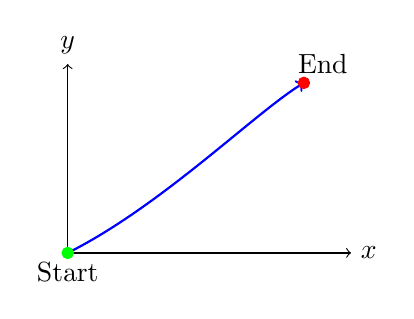
\begin{tikzpicture}[scale=1.2]
        % Axes
        \draw[->] (0,0) -- (3,0) node[right] {$x$};
        \draw[->] (0,0) -- (0,2) node[above] {$y$};
        % Trajectory
        \draw[thick,blue,->] (0,0) .. controls (1,0.5) and (2,1.5) .. (2.5,1.8);
        % Start and end
        \filldraw[green] (0,0) circle (0.06);
        \filldraw[red] (2.5,1.8) circle (0.06);
        \node at (0,-0.2) {Start};
        \node at (2.7,2) {End};
    \end{tikzpicture}
    \end{center}
    \small{(Example: Robot follows a curved path as it moves and turns)}
\end{frame}

\begin{frame}
    \frametitle{Trajectory Example}
    \textbf{Given:} $v = 0.25$ m/s, $\omega = 0.2$ rad/s, $x(0) = 0$, $y(0) = 0$, $\theta(0) = 0$
    \begin{itemize}
        \item $x(10) = 0 + 0.25 \times \cos(0) \times 10 = 2.5$ m
        \item $y(10) = 0 + 0.25 \times \sin(0) \times 10 = 0$ m
        \item $\theta(10) = 0 + 0.2 \times 10 = 2$ rad
    \end{itemize}
    \textbf{Interpretation:} After 10 seconds, the robot has moved forward and rotated.
\end{frame}

\begin{frame}
    \frametitle{Practical Considerations}
    \begin{itemize}
        \item Wheel slip and real-world effects
        \item Sensor noise
        \item Model limitations (e.g., cannot move sideways)
    \end{itemize}
    \textbf{Always validate models with experiments!}
\end{frame}

\begin{frame}
    \frametitle{Summary and Q\&A}
    \begin{itemize}
        \item Recap of kinematic models and equations
        \item Applications in mobile robotics
        \item Questions and discussion
    \end{itemize}
\end{frame}

\end{document}